\documentclass[aspectratio=169,11pt]{beamer}
\usetheme{Madrid}
\usecolortheme{beaver}
\setbeamertemplate{navigation symbols}{}
\usepackage{booktabs}
\usepackage{graphicx}
\graphicspath{{figures/}}

\title[Distributed LLM Inference on the Edge]{Distributed LLM Inference on the Edge}
\subtitle{Running Llama-3.2-3B on a cluster of Raspberry Pis}
\author[Group 7]{Yuzhou Zhang \and Yunfan Zhang \and Shuo Zhang \and Wenqi Zhao}
\institute[Chalmers]{DAT300/DIT616 -- Group 7\\Supervisors: Yixing Zhang, Romaric Duvignau}
\date[Oct 2026]{Final presentation, October 2026}

\begin{document}

\begin{frame}
\titlepage
\end{frame}

\begin{frame}{Outline}
\tableofcontents
\end{frame}

\section{Background}

\begin{frame}{Why run an LLM on edge devices?}
\begin{columns}[T]
\column{0.48\textwidth}
\begin{itemize}
\item Cloud LLMs send your data away and need a connection
\item One Raspberry Pi can run a small model, but slowly
\item Can several cheap boards work together and be faster?
\end{itemize}
\column{0.48\textwidth}
Research questions
\begin{enumerate}
\item How does speed scale with the number of nodes?
\item Pipeline or tensor parallelism?
\item What is the bottleneck?
\item Can we fix it without losing accuracy?
\end{enumerate}
\end{columns}
\vspace{6mm}
\centering Model: Llama-3.2-3B-Instruct, 4-bit (1.9 GB)
\end{frame}

\begin{frame}{Our cluster}
\begin{columns}[c]
\column{0.6\textwidth}
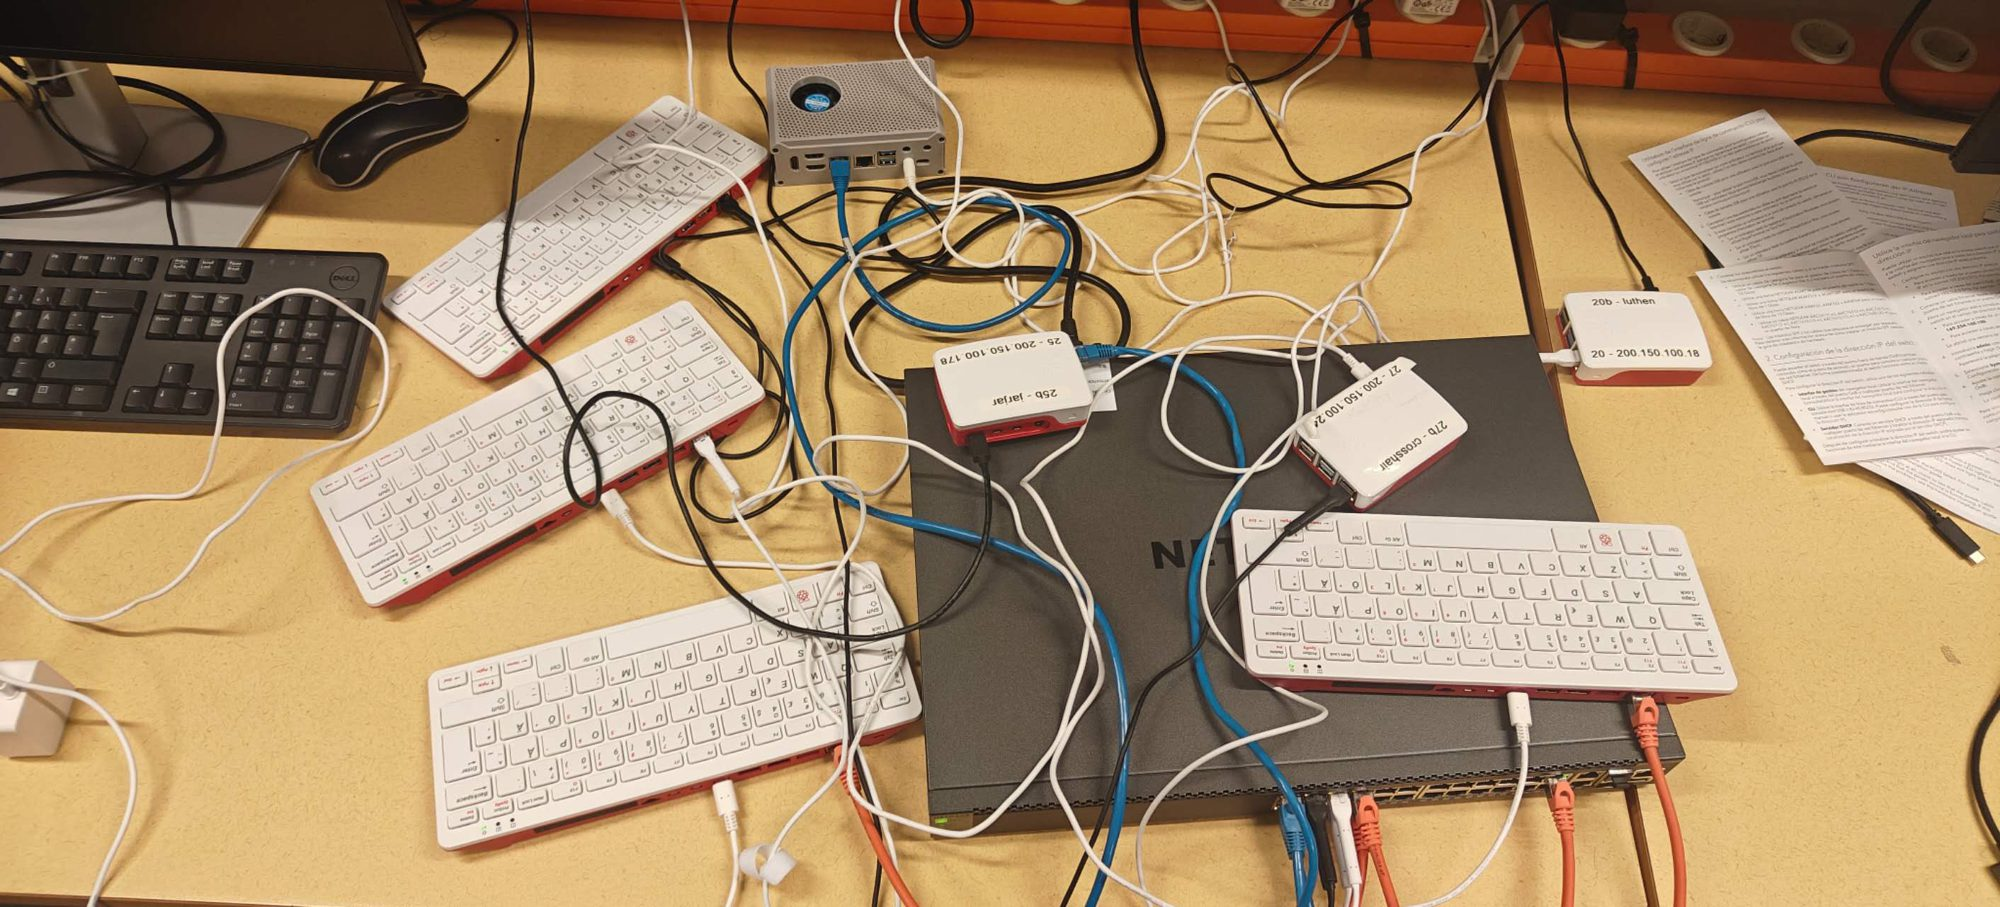
\includegraphics[width=\textwidth]{cluster_photo.jpg}
\column{0.38\textwidth}
\begin{itemize}
\item 7 Raspberry Pis (Pi 400 and Pi 4B)
\item 1 LubanCat-5 board (RK3588)
\item One Gigabit switch
\end{itemize}
\vspace{3mm}
\scriptsize
\begin{tabular}{@{}lcc@{}}
\toprule
 & Pi & RK3588 \\
\midrule
Mem.\ bandwidth & 4 GB/s & 22 GB/s \\
Decode, alone & 1.84 tok/s & 12.28 tok/s \\
\bottomrule
\end{tabular}
\end{columns}
\end{frame}

\begin{frame}{How we ran and measured it}
\begin{columns}[c]
\column{0.5\textwidth}
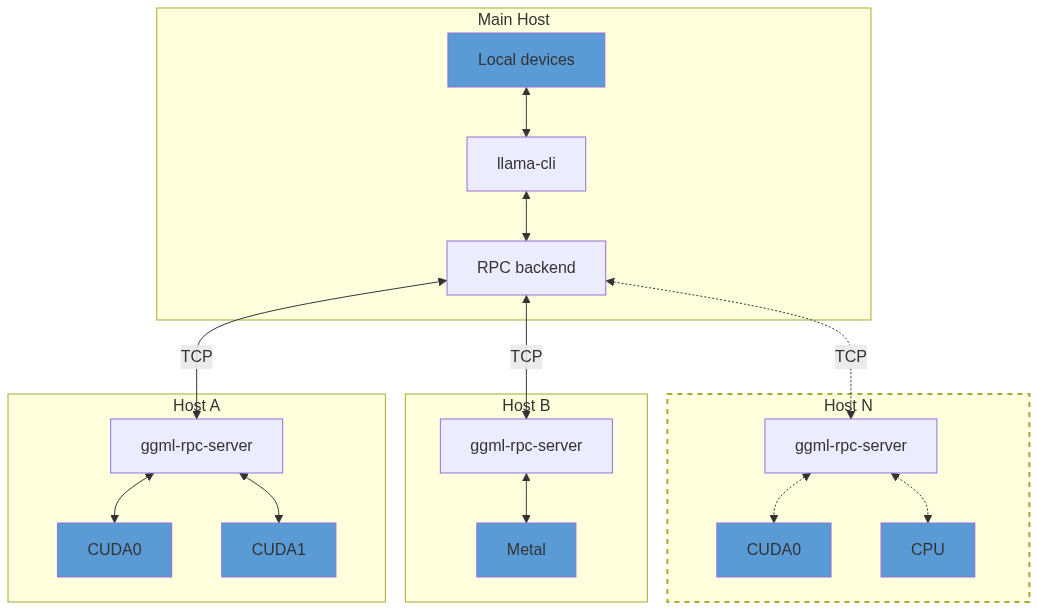
\includegraphics[width=\textwidth]{llamacpp_rpc_official.png}
{\scriptsize llama.cpp RPC backend (from the official docs)}
\column{0.48\textwidth}
\begin{itemize}
\item Baseline: Distributed Llama, 1/2/4 nodes
\item Then llama.cpp RPC with 1--8 devices
\begin{itemize}
\item pipeline parallel (PP): split by layers
\item tensor parallel (TP): split every layer
\end{itemize}
\item To find bottlenecks we logged
\begin{itemize}
\item CPU, memory and network on every device
\item time spent per RPC command
\end{itemize}
\end{itemize}
\end{columns}
\end{frame}

\section{Results and bottlenecks}

\begin{frame}{Decode speed from 1 to 8 nodes}
\begin{columns}[c]
\column{0.6\textwidth}
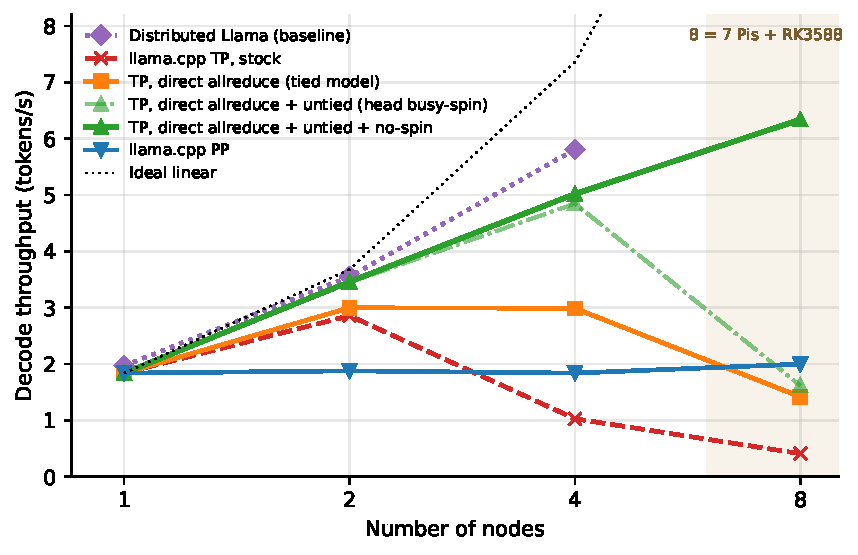
\includegraphics[width=\textwidth]{decode_scaling.pdf}
\column{0.38\textwidth}
\begin{itemize}
\item PP is never faster than one Pi
\item Stock TP gets \emph{slower} with more nodes (0.41 tok/s on 8)
\item After our changes: 6.34 tok/s on 8 nodes, 3.4$\times$ one Pi
\end{itemize}
\vspace{2mm}
Three bottlenecks explain the gap.
\end{columns}
\end{frame}

\begin{frame}{Bottleneck 1: all traffic goes through the head}
\begin{columns}[c]
\column{0.5\textwidth}
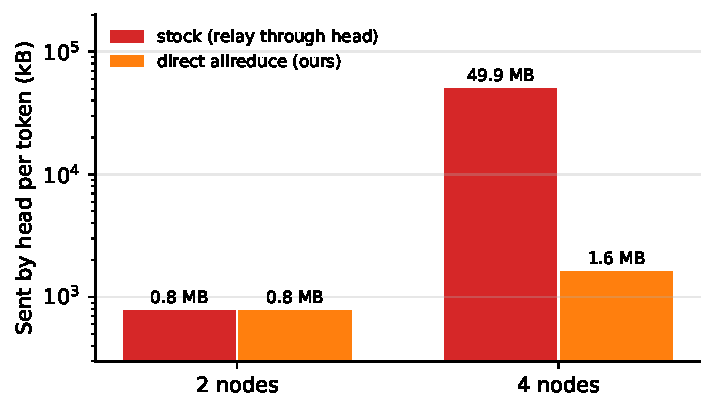
\includegraphics[width=\textwidth]{head_traffic.pdf}
\column{0.48\textwidth}
\begin{itemize}
\item With more than 2 nodes, the head collects and redistributes every partial sum
\item On 4 nodes the head sends about 50 MB per token
\item We added a direct allreduce between the nodes ($\log_2 N$ steps)
\item 4 nodes: 1.03 to 2.99 tok/s
\end{itemize}
\end{columns}
\end{frame}

\begin{frame}{Bottleneck 2: the output layer is not split}
\begin{columns}[c]
\column{0.58\textwidth}
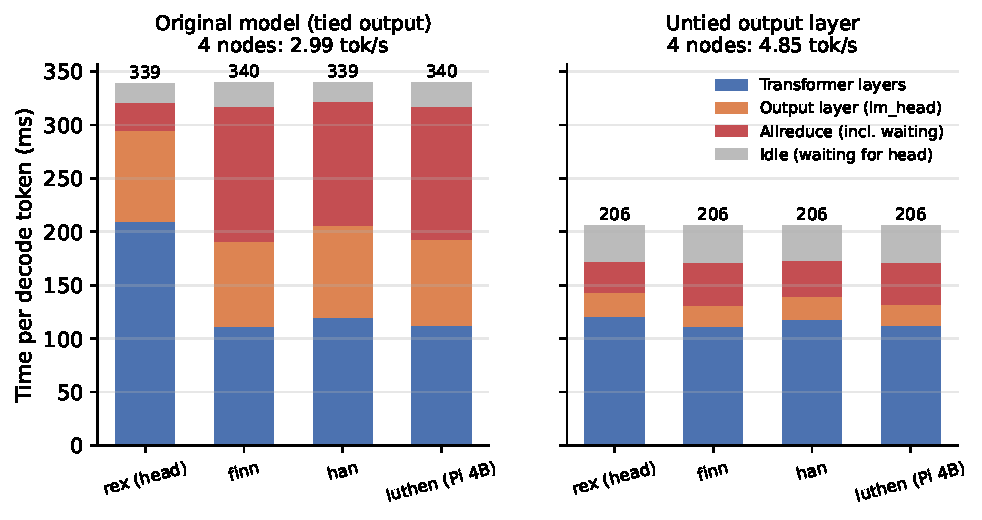
\includegraphics[width=\textwidth]{trace_breakdown_tp4.pdf}
\column{0.4\textwidth}
\begin{itemize}
\item The timing log showed 80--85 ms per token on the output layer on \emph{every} node
\item Llama-3.2 shares it with the input embedding, so llama.cpp copies it instead of splitting it
\item We saved a separate copy in the model file (same output, same perplexity)
\item 4 nodes: 2.99 to 4.85 tok/s
\end{itemize}
\end{columns}
\end{frame}

\begin{frame}{Bottleneck 3: the head's CPU at 8 nodes}
\begin{columns}[c]
\column{0.58\textwidth}
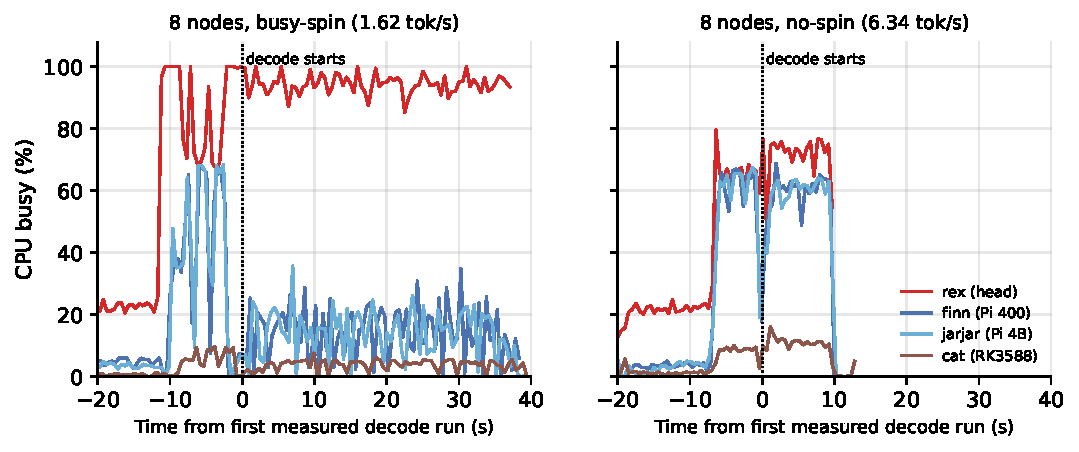
\includegraphics[width=\textwidth]{cpu_timeline_tp8.pdf}
\column{0.4\textwidth}
\begin{itemize}
\item Head CPU 94\%, workers only 15\%
\item Workers waited 470 of 631 ms per token
\item With gdb we found 8 threads busy-waiting on the head's 4 cores
\item We added an option to let them sleep instead
\item 8 nodes: 1.62 to 6.34 tok/s
\end{itemize}
\end{columns}
\end{frame}

\begin{frame}{Is the network the bottleneck?}
\begin{columns}[c]
\column{0.6\textwidth}
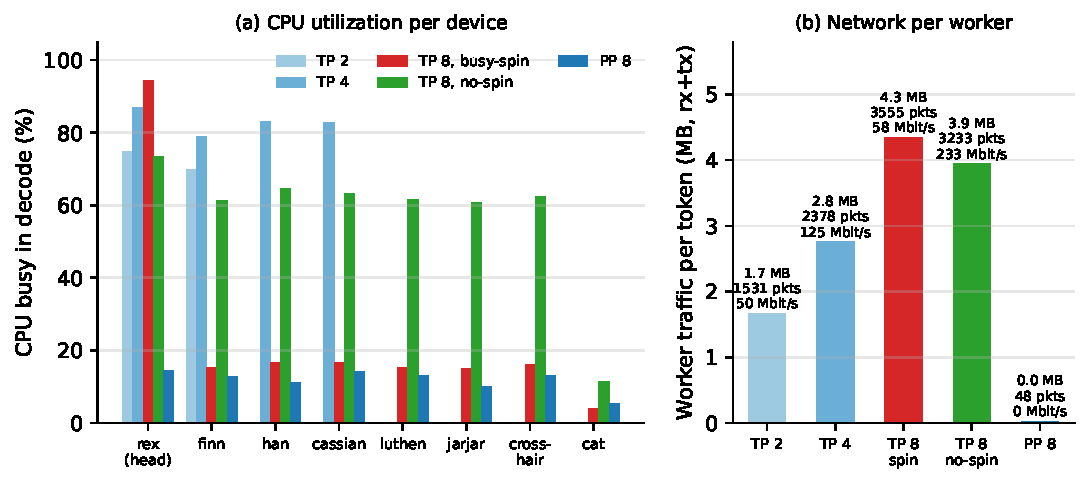
\includegraphics[width=\textwidth]{resources_decode.pdf}
\column{0.38\textwidth}
\begin{itemize}
\item On Gigabit: no. Each worker uses at most 233 of 940 Mbit/s
\item Fixing bottleneck 3 made it 3.9$\times$ faster with the \emph{same} traffic
\item One Pi alone is limited by memory bandwidth
\end{itemize}
\end{columns}
\end{frame}

\begin{frame}{What if the network is slow? (10 Mbit/s)}
\begin{columns}[c]
\column{0.58\textwidth}
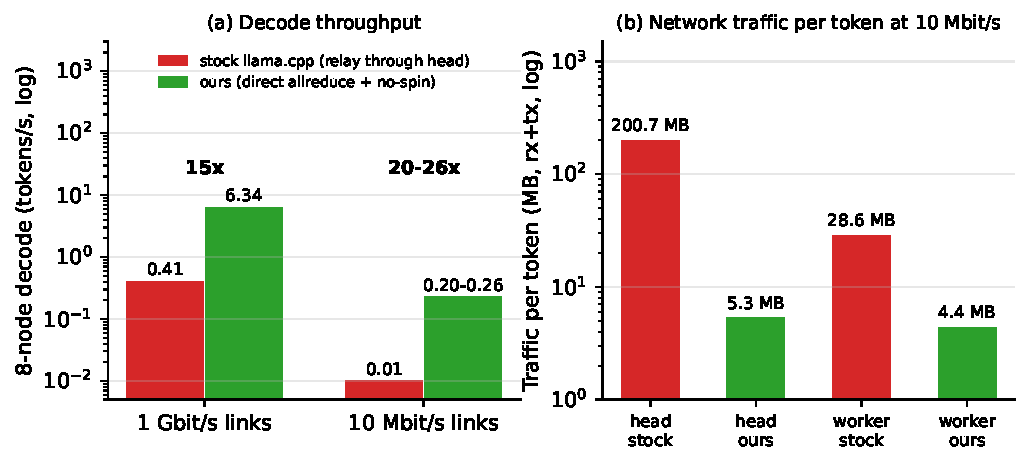
\includegraphics[width=\textwidth]{bandwidth_10mbps.pdf}
\column{0.4\textwidth}
\begin{itemize}
\item We limited all 8 devices to 10 Mbit/s
\item Stock: 200 MB per token through the head, 0.01 tok/s
\item Ours: 5.3 MB, 0.20--0.26 tok/s
\item 20--26$\times$ faster here vs.\ 15$\times$ on Gigabit
\end{itemize}
\end{columns}
\end{frame}

\begin{frame}{Pipeline parallelism and a faster board}
\begin{columns}[T]
\column{0.5\textwidth}
\centering
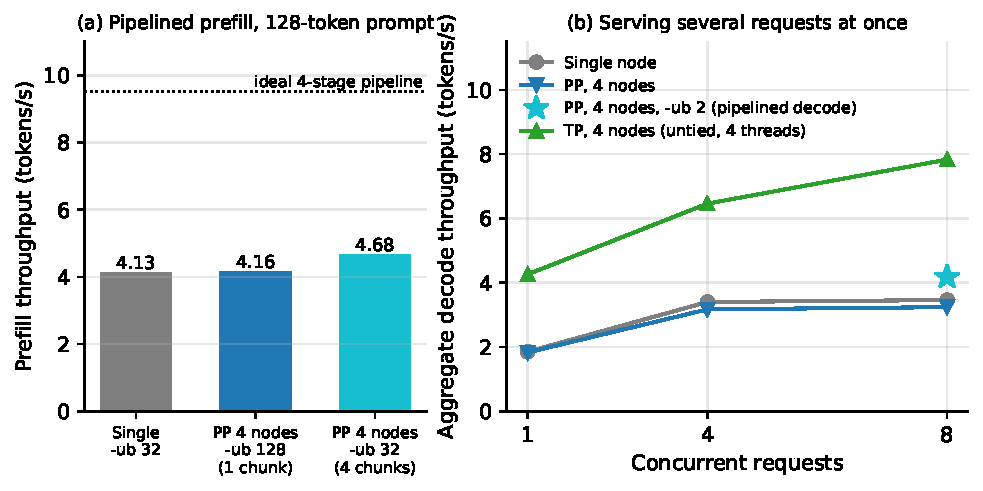
\includegraphics[width=\textwidth]{pp_pipeline_batching.pdf}
\begin{itemize}\footnotesize
\item PP only helps with several requests at once (+29\%)
\item Its real use: models that don't fit on one board
\end{itemize}
\column{0.5\textwidth}
\centering
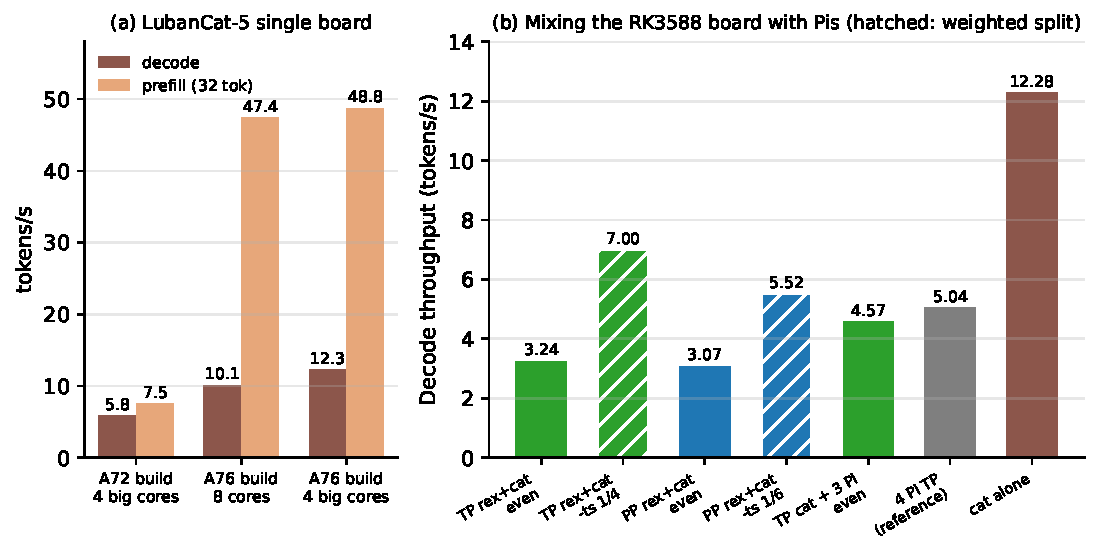
\includegraphics[width=\textwidth]{heterogeneous.pdf}
\begin{itemize}\footnotesize
\item Compiling for the RK3588's CPU: 5.84 to 12.28 tok/s
\item Giving it a bigger share helps (TP on 2 nodes: 3.24 to 7.00)
\item But it alone beats the whole Pi cluster for this model
\end{itemize}
\end{columns}
\end{frame}

\section{Conclusion}

\begin{frame}{Problems we ran into}
\begin{itemize}
\item The switch lost its DHCP settings after a reset, so we gave every board a static IP
\item One Pi rebooted mid-test because of a weak power supply
\item The Pis have no real-time clock, so we corrected clock offsets before comparing logs
\item Our first monitoring script (shell) slowed decoding by 5\%; a small C program fixed this
\item Uneven splits on 8 nodes fall back to the slow path, so we left them out
\end{itemize}
\end{frame}

\begin{frame}{Conclusions and future work}
\begin{columns}[T]
\column{0.55\textwidth}
\begin{enumerate}
\item TP scales to 3.4$\times$ on 8 Pis; PP does not speed up a single request
\item TP needs far more communication than PP
\item The limits were the head relay, the unsplit output layer and the head's CPU, not network bandwidth
\item Three small changes, no accuracy loss
\end{enumerate}
\column{0.42\textwidth}
Future work
\begin{itemize}
\item Uneven splits for mixed devices
\item Models too large for one board
\item Fewer sync rounds per token
\end{itemize}
\end{columns}
\end{frame}

\begin{frame}
\centering\Large Thank you! Questions?

\vfill
{\tiny\color{gray} Code and data: \url{https://github.com/44sunsetsf/dat300-edge-llm}}
\end{frame}

\end{document}
